\documentclass{article}
\usepackage{graphicx}
\usepackage{placeins}
\usepackage{amsmath}
\usepackage{listings}
\usepackage{xcolor}

\title{Factorio Planning}
\author{Anton Althoff}
\date{March 2026}

\newcommand{\factorio}[1]{\textit{#1}}

% ASP Code Styling
\lstdefinelanguage{asp}{
  morecomment=[l]{\%},
  morestring=[b]",
  alsoletter={_},
  sensitive=true,
  keywords={item,crafting,building,dur,building_cost,crafting_cost,crafting_out,
            building_in,building_out,init_global_stock,init_local_stock,
            init_building_count,init_local_cap,init_global_cap,
            goal_item,goal_building,time,step,zone,slot,next_zone,available_index,
            slot_map,has_assignment,can_build,stock,global_stock,building_count,
            act,busy,finish,finish_any_craft_for,uses_build_resource,uses_craft_resource,
            cost_build,cost_craft,yield_craft,local_available,global_available,
            local_space,global_space,slot_utilization,input_from_local,input_from_global,
            output_to_local,output_to_global},
}
\lstset{
  basicstyle=\ttfamily\small,
  columns=fullflexible,
  frame=single,
  breaklines=true,
  keywordstyle=\color{blue!60!black},
  commentstyle=\color{green!40!black},
  stringstyle=\color{orange!60!black},
  showstringspaces=false
}

\begin{document}

\maketitle

\section{Introduction}
\factorio{Factorio} is an automation game centered around building a factory. Starting from a set of raw resources found on the map such as iron, copper, coal, and stone, the player iteratively constructs a production system that transforms these basic materials into increasingly complex intermediates and final products, with the goal of building a rocket to escape the planet.

The core challenge of \factorio{Factorio} is fundamentally a planning problem: the player must anticipate demand, balance production chains, and avoid bottlenecks. While the game is spatial (placement of buildings and routing of conveyor belts is an important aspect), this project focuses on the temporal scheduling and resource-flow aspects. We therefore abstract away the 2D geometry and aim to model the game in a simplified manner that still preserves most of the core mechanics. The resulting model can be used find viable action sequences to reach set goals given a game instance. 

\section{Background}
To model \textit{Factorio}, we must first highlight the core game mechanics.
\subsection{Production and crafting}
Resources are transformed according to a set of recipes. A recipe has a set of input items, a set of output items, and a duration. These recipes can be executed either manually by the player or automatically by machines.

Manual crafting is flexible, since it does not require existing infrastructure, but it is highly limited in throughput since the player can only craft one recipe at a time. As a result, manual crafting is mainly useful in the early stages of the game or for low-volume recipes. Meaningful progress is only feasible with automation.

\subsection{Automation through buildings}
Automation is achieved by constructing buildings that transform items according to a specific recipe. Once placed, buildings operate in parallel and provide the throughput necessary for large-scale production.

From a planning perspective, each building type is a production unit with:
\begin{itemize}
    \item a \textbf{construction cost}, i.e.\ the items required to build it,
    \item a set of \textbf{input requirements} consumed while operating,
    \item a set of \textbf{outputs} produced while operating,
    \item and a limited \textbf{capacity}, determined by how many such buildings have been constructed.
\end{itemize}
Notably, available capacity does not guarantee actual production: a machine can only run if its required inputs are available and if there is sufficient storage space for its outputs.

\subsection{Logistics and bottlenecks}
A large part of the difficulty of \factorio{Factorio} lies in logistics. Resources must be moved between buildings using belts, inserters, pipes, or similar infrastructure. In the full game, this introduces spatial constraints, transport delays, and throughput limits. Even when the necessary items exist somewhere in the factory, production can stall because the right items do not reach the right machines at the right time.

%We abstract away from explicit geometry and transport networks, but try to preserve the resource competition and local bottleneck aspects of the game. Buildings do not draw an item pool in an arbitrary way; instead, resource availability is structured so that shortages in one part of the factory can restrict downstream production.

\subsection{Technological progression}
Progression in \factorio{Factorio} is gated by research. New technologies are unlocked by producing science packs and processing them in laboratories. Research expands the set of available recipes and buildings, allowing the player to move from early-game production to more advanced outputs.

\section{Modeling}
%TODO rewrite
We model \factorio{Factorio} as a discrete-time planning problem in Answer Set Programming (ASP). Our abstraction focuses on the temporal scheduling of building and crafting actions. We abstract away from the logistic aspects of the game, instead we introduce a structured notion of factory regions, called \textbf{zones}. Technological progression through research is also not modeled. The full code can be found in the files \textbf{model.lp}, \textbf{game.lp}, and \textbf{instances/*.lp}.

%TODO we dont model tech progression, logistic, spatial

\subsection{Static game encoding}
All game knowledge is represented as facts. This makes the model easy to extend with additional recipes, items, and buildings.

The encoding distinguishes between \textbf{crafting recipes}, which can be executed manually by the player, and \textbf{buildings} representing automated production units. Items, recipes, durations, inputs, and outputs are all declared declaratively.

\begin{lstlisting}[label=lst:game_encoding,language=asp,caption={Excerpt of game encoding (game.lp).}]
% items
item(iron_plate).
item(iron_gear).
item(green_circuit).
item(assembler).

% manual crafting recipe
crafting(assembler).
dur(assembler,1).
crafting_cost(assembler, iron_plate, 100).
crafting_cost(assembler, iron_gear, 50).
crafting_cost(assembler, green_circuit, 30).
crafting_out(assembler, assembler, 10).

% automated building
building(green_circuit_assembler).
dur(green_circuit_assembler, 1).
building_cost(green_circuit_assembler, assembler, 5).
building_in(green_circuit_assembler, iron_plate, 100).
building_in(green_circuit_assembler, copper_cable, 300).
building_in(green_circuit_assembler, electricity, 78).
building_out(green_circuit_assembler, green_circuit, 100).
\end{lstlisting}

The static game encoding can be found in \textbf{game.lp}.

\subsection{Simplifications}
The model uses fixed-length time horizons, typically between 20 and 30 steps, where each step corresponds to 30 seconds of in-game time. To make modeling of the game feasible, we set the following assumptions and simplifications:
\begin{itemize}
    \item Spatial placement is abstracted away and replaced by zones.
    \item Logistic infrastructure is not modeled explicitly.
    \item All recipes are available from the start, not gated behind research.
    \item Recipes are treated at aggregate rates per step.
    \item The player can initiate at most one manual crafting action and one building action per step.
\end{itemize}
These simplifications reduce complexity while keeping the planning structure that makes the game interesting.

\subsection{Actions}
At each step, the player may start up to one crafting action and one building action. These actions are not instantaneous. Once started, they occupy the respective activity channel for a number of steps given by \texttt{dur(\dots)}. While a channel is occupied, no other action of the same type can be started.

\begin{lstlisting}[label=lst:actions_clean,language=asp,caption={Action selection and delayed completion (model.lp).}]
% at most one craft and one build action per step
0 { act(craft(C), STEP) : crafting(C), dur(C, _) } 1 :- step(STEP), not busy(craft, STEP).

0 { act(build(B, Z), STEP) : building(B), zone(Z), dur(B, _), can_build(B, Z) } 1 :- step(STEP), not busy(build, STEP).

% activity channels stay occupied until the duration expires
busy(craft, STEP) :- step(STEP), act(craft(C), STEP0), dur(C, D), STEP > STEP0, STEP < STEP0 + D.

busy(build, STEP) :- step(STEP), act(build(B, Z), STEP0), dur(B, D), STEP > STEP0, STEP < STEP0 + D.

% completion time
finish(craft(C), TIME) :- time(TIME), act(craft(C), STEP0), dur(C, D), TIME = STEP0 + D.

finish(build(B, Z), TIME) :- time(TIME), act(build(B, Z), STEP0), dur(B, D), TIME = STEP0 + D.
\end{lstlisting}

Starting an action immediately consumes its required input items from the global stock. A completed craft yields items when the crafting duration has passed, and a completed build increases production capacity from the time point after finishing.

\subsection{Zones, slots, and production capacity}
\FloatBarrier
To preserve some notion of locality without modeling full geometry, the factory is partitioned into \textbf{zones} (Figure~\ref{fig:zones}). Each zone contains a fixed number of \textbf{slots}. A slot may be assigned at most one building type, and a building type may appear in at most one slot per zone.

\begin{figure}
    \centering
    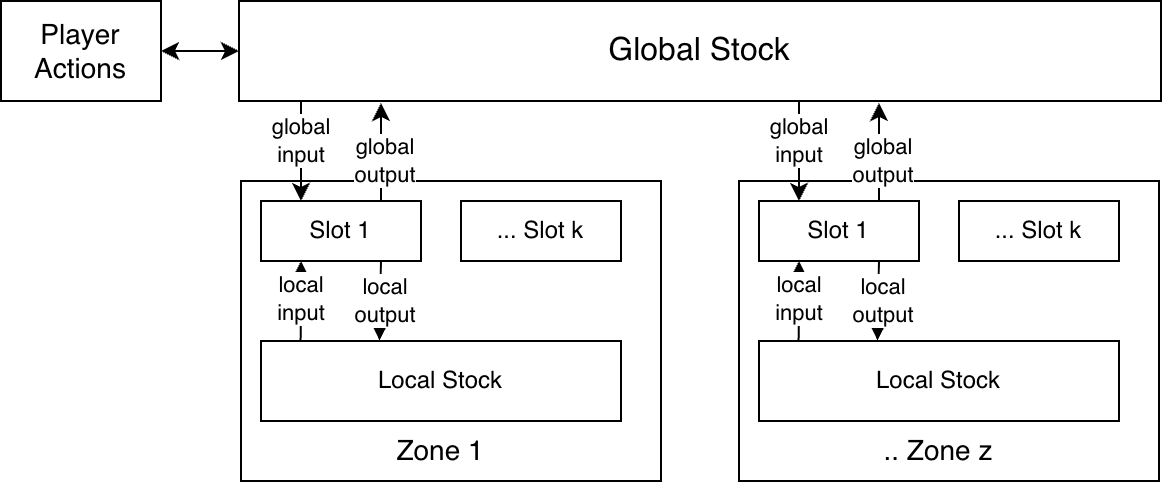
\includegraphics[width=1\linewidth]{images/zones_new.png}
    \caption{Zone resource flow model.}
    \label{fig:zones}
\end{figure}

The slot assignment does not change over the entire horizon. What does change is the number of buildings \texttt{building\_count(B,Z,T)} of a given type in a zone, which represents the maximum production capacity. In the implementation, the initial slot assignment can be chosen by the solver or induced by \texttt{init\_building\_count(B,Z,S,Count)}: if a building type has a positive initial count in slot $S$, then that slot is associated with that building type.
\FloatBarrier
\begin{lstlisting}[label=lst:zones_clean,language=asp,caption={Zone and slot structure (model.lp).}]
zone(1..num_zones).
slot(1..num_slots).
available_index(1..num_slots+1).
next_zone(Z, Z+1) :- zone(Z), zone(Z+1).

% at most one building type per slot
0 { slot_map(Z, S, B) : building(B) } 1 :- zone(Z), slot(S).

% a building type may occupy at most one slot per zone
:- slot_map(Z, S1, B), slot_map(Z, S2, B), S1 != S2.

% keep used slots left-aligned
has_assignment(Z, S) :- slot_map(Z, S, _).
:- has_assignment(Z, S+1), not has_assignment(Z, S), slot(S).

% build actions only for assigned building types
can_build(B, Z) :- building(B), zone(Z), slot_map(Z, _, B).

% state variables
&dom{0..max_val} = stock(I,Z,T) :- item(I), zone(Z), time(T).
&dom{0..max_val} = global_stock(I,T) :- item(I), time(T).
&dom{0..max_val} = building_count(B,Z,T) :- building(B), zone(Z), time(T).

% unassigned building types have zero capacity
&sum { building_count(B, Z, T) } = 0 :- building(B), zone(Z), time(T), not can_build(B, Z).
\end{lstlisting}

\subsection{Time model and state variables}
We model the factory as a system with discrete states over a fixed horizon $H$, with
\[
\texttt{time}(0..H), \qquad \texttt{step}(0..H-1).
\]
A \textbf{time point} represents a snapshot of the game state, while a \textbf{step} represents the transition between two consecutive snapshots. Intuitively, the order is
\[
\text{Time }0 \;\vert\; \text{Step }0 \;\vert\; \text{Time }1 \;\vert\; \text{Step }1 \;\vert\; \cdots \;\vert\; \text{Time }H.
\]
One step corresponds to 30 seconds of in-game time.

At each time point $T$, the relevant part of the state is given by:
\begin{itemize}
    \item \texttt{global\_stock(I,T)}: the global stock of item $I$,
    \item \texttt{stock(I,Z,T)}: the local stock of item $I$ in zone $Z$,
    \item \texttt{building\_count(B,Z,T)}: the number of buildings of type $B$ in zone $Z$.
\end{itemize}
The transition from time $T$ to $T+1$ is driven by the chosen actions, the utilization of buildings during step $T$, and the resulting resource flows.

\subsection{Intra-step resource allocation}
A central difficulty of the model is that, within one step, multiple buildings may compete for the same limited resources. To remove ambiguity in how limited resources are shared, we fix the order in which zones and slots get access to the available resources. This ordering determines which allocations are feasible: later slots can only use what remains after earlier slots’ chosen consumption. In our model, utilization is not forced to be greedy, but selected by the solver subject to the aforementioned constraints and to later optimization objectives, since forcing maximal utilization per slot increased solve time and memory requirements to the point of infeasibility. Resource allocation follows the sequence
\[
(z_1,s_1) \rightarrow (z_1,s_2) \rightarrow \cdots \rightarrow (z_2,s_1) \rightarrow \cdots
\]
where $(z,s)$ corresponds to slot $s$ in zone $z$.

At the beginning of a step, manual crafting and building actions may consume items from the global stock. The remaining global stock is then made available to the first slot of the first zone. Similarly, the first slot in each zone has the full local stock available for consumption (Listing~\ref{lst:flow_init}). The same idea is used for output space: both local and global storage capacities in combination with the respective stock levels determine the amount of space left for output items.

\begin{lstlisting}[language=asp,caption={Initialization of per-step resource availability and action costs (model.lp).},label={lst:flow_init}]
uses_build_resource(I, T) :- act(build(B, _), T), building_cost(B, I, _).
uses_craft_resource(I, T) :- act(craft(C), T), crafting_cost(C, I, _).

% cost of building/crafting
&dom{0..max_val} = cost_build(I, T) :- item(I), step(T).
&dom{0..max_val} = cost_craft(I, T) :- item(I), step(T).

&sum { cost_build(I, T) } = Qty :- step(T), item(I), act(build(B, _), T), building_cost(B, I, Qty).
&sum { cost_build(I, T) } = 0 :- step(T), item(I), not uses_build_resource(I, T).
&sum { cost_craft(I, T) } = Qty :- step(T), item(I), act(craft(C), T), crafting_cost(C, I, Qty).
&sum { cost_craft(I, T) } = 0 :- step(T), item(I), not uses_craft_resource(I, T).

&dom{0..max_val} = local_available(I, Z, IDX, T) :- item(I), zone(Z), available_index(IDX), step(T).
&dom{0..max_val} = global_available(I, Z, IDX, T) :- item(I), zone(Z), available_index(IDX), step(T).
&dom{0..max_val} = local_space(I, Z, IDX, T) :- item(I), zone(Z), available_index(IDX), step(T).
&dom{0..max_val} = global_space(I, Z, IDX, T) :- item(I), zone(Z), available_index(IDX), step(T).

% each zone starts with its local stock available to slot 1
&sum { local_available(I, Z, 1, T); -stock(I, Z, T) } = 0 :- item(I), zone(Z), step(T).

% first slot of first zone receives remaining global stock
&sum { global_available(I, 1, 1, T); -global_stock(I, T); cost_build(I, T); cost_craft(I, T) } = 0 :- item(I), step(T).

% available output space
&sum { local_space(I, Z, 1, T); stock(I, Z, T) } = Cap :- item(I), zone(Z), step(T), init_local_cap(I, Z, Cap).
&sum { local_space(I, Z, 1, T) } = max_val :- item(I), zone(Z), step(T), not init_local_cap(I, Z, _).
&sum { global_space(I, 1, 1, T); global_stock(I, T) } = Cap :- item(I), step(T), init_global_cap(I, Cap).
&sum { global_space(I, 1, 1, T) } = max_val :- item(I), step(T), not init_global_cap(I, _).
\end{lstlisting}

For each occupied slot, the model chooses a \textbf{utilization} value. This value is bounded between zero and the capacity, i.e., the building count of the assigned building type. It is then further constrained by available inputs and available output space. Utilization captures the actual production rate of a slot during a step, and \texttt{building\_count} represents its maximum possible production capacity.

For each required input item, the total amount drawn from local and global stock must match recipe demand multiplied by utilization; similarly, the total amount sent to local and global output buffers must match recipe output multiplied by utilization. The model ensures that no slot can consume more than what is currently available or produce more than what can be stored (Listing~\ref{lst:intrastep_flow}).

\begin{lstlisting}[language=asp,caption={Core intra-step flow constraints for one slot (model.lp).},label={lst:intrastep_flow}]
&dom{0..max_val} = slot_utilization(Z, S, T) :- zone(Z), slot(S), step(T).

% utilization cannot exceed installed capacity
&sum { slot_utilization(Z, S, T); -building_count(B, Z, T) } <= 0 :- slot_map(Z, S, B), step(T).
&sum { slot_utilization(Z, S, T) } = 0 :- zone(Z), slot(S), step(T), not has_assignment(Z, S).

% empty slots or irrelevant items have zero flow
&sum { input_from_local(I, Z, S, T) } = 0 :- item(I), zone(Z), slot(S), step(T), not has_assignment(Z, S).
&sum { input_from_global(I, Z, S, T) } = 0 :- item(I), zone(Z), slot(S), step(T), not has_assignment(Z, S).
&sum { output_to_local(I, Z, S, T) } = 0 :- item(I), zone(Z), slot(S), step(T), not has_assignment(Z, S).
&sum { output_to_global(I, Z, S, T) } = 0 :- item(I), zone(Z), slot(S), step(T), not has_assignment(Z, S).

&sum { input_from_local(I, Z, S, T) } = 0 :- slot_map(Z, S, B), not building_in(B, I, _), step(T), item(I).
&sum { input_from_global(I, Z, S, T) } = 0 :- slot_map(Z, S, B), not building_in(B, I, _), step(T), item(I).
&sum { output_to_local(I, Z, S, T) } = 0 :- slot_map(Z, S, B), not building_out(B, I, _), step(T), item(I).
&sum { output_to_global(I, Z, S, T) } = 0 :- slot_map(Z, S, B), not building_out(B, I, _), step(T), item(I).

% required inputs = recipe demand * utilization
&sum { input_from_local(I, Z, S, T); input_from_global(I, Z, S, T); -Qty*slot_utilization(Z, S, T) } = 0 :- slot_map(Z, S, B), building_in(B, I, Qty), step(T).

% produced outputs = recipe output * utilization
&sum { output_to_local(I, Z, S, T); output_to_global(I, Z, S, T); -Qty*slot_utilization(Z, S, T) } = 0 :- slot_map(Z, S, B), building_out(B, I, Qty), step(T).

% cannot consume more than available
&sum { input_from_local(I, Z, S, T); -local_available(I, Z, S, T) } <= 0 :- item(I), zone(Z), slot(S), step(T).
&sum { input_from_global(I, Z, S, T); -global_available(I, Z, S, T) } <= 0 :- item(I), zone(Z), slot(S), step(T).

% cannot produce more than available storage space
&sum { output_to_local(I, Z, S, T); -local_space(I, Z, S, T) } <= 0 :- item(I), zone(Z), slot(S), step(T).
&sum { output_to_global(I, Z, S, T); -global_space(I, Z, S, T) } <= 0 :- item(I), zone(Z), slot(S), step(T).
\end{lstlisting}

After the utilization of a slot is fixed, the remaining local resources, global resources, and output space are passed forward. 
\begin{lstlisting}[language=asp,caption={Propagation of remaining resources to the next slot and next zone (model.lp).},label={lst:flow_propagation}]
% pass remaining resources to next slot
&sum { local_available(I, Z, S+1, T); -local_available(I, Z, S, T); input_from_local(I, Z, S, T) } = 0 :- item(I), zone(Z), slot(S), step(T).

&sum { global_available(I, Z, S+1, T); -global_available(I, Z, S, T); input_from_global(I, Z, S, T) } = 0 :- item(I), zone(Z), slot(S), step(T).

% pass remaining output space to next slot
&sum { local_space(I, Z, S+1, T); -local_space(I, Z, S, T); output_to_local(I, Z, S, T) } = 0 :- item(I), zone(Z), slot(S), step(T).

&sum { global_space(I, Z, S+1, T); -global_space(I, Z, S, T); output_to_global(I, Z, S, T) } = 0 :- item(I), zone(Z), slot(S), step(T).

% after the last slot of zone Z, the remaining global pool is passed to zone Z+1
&sum { global_available(I, Znext, 1, T); -global_available(I, Z, num_slots+1, T) } = 0 :- item(I), next_zone(Z, Znext), step(T).
&sum { global_space(I, Znext, 1, T); -global_space(I, Z, num_slots+1, T) } = 0 :- item(I), next_zone(Z, Znext), step(T).
\end{lstlisting}

\subsection{State transition}
Once all slots have been processed for step $T$, the model fixes the state at time $T+1$. The remaining stock after consumption is carried forward, and all outputs produced during the step are added.

For local stock, the update rule is:
\[
\text{stock}_{T+1}
=
\text{stock\_local\_remaining}_T
+
\text{output\_to\_local}_T.
\]
For global stock, the same rule applies, with the addition of the items obtained from finished crafting actions. Building and crafting costs do not appear explicitly because they were already deducted at the beginning of the respective step through \texttt{global\_available}. Listing~\ref{lst:interstep_transition} shows the transition equations.

\begin{lstlisting}[language=asp,caption={Inter-step conservation and state transition (model.lp).},label={lst:interstep_transition}]
% building capacity increases when build action finishes
&sum { building_count(B, Z, T+1); -building_count(B, Z, T) } = 1 :- building(B), zone(Z), step(T), slot_map(Z, _, B), finish(build(B, Z), T).
&sum { building_count(B, Z, T+1); -building_count(B, Z, T) } = 0 :- building(B), zone(Z), step(T), slot_map(Z, _, B), not finish(build(B, Z), T).

% local stock at T+1 = remaining local availability + outputs sent to local stock
&sum { stock(I, Z, T+1); -local_available(I, Z, num_slots+1, T); -output_to_local(I, Z, S, T) : slot(S) } = 0 :- item(I), zone(Z), step(T).

% completed crafts yield new items
&dom{0..max_val} = yield_craft(I, T) :- item(I), step(T).
&sum { yield_craft(I, T) } = Qty :- time(T), item(I), finish(craft(C), T), crafting_out(C, I, Qty).
&sum { yield_craft(I, T) } = 0 :- time(T), item(I), not finish_any_craft_for(I, T).

% global stock at T+1 = remaining global availability + outputs to global + finished craft yield
&sum { global_stock(I, T+1); -global_available(I, num_zones, num_slots+1, T); -output_to_global(I, Z, S, T) : zone(Z), slot(S); -yield_craft(I, T+1) } = 0 :- item(I), step(T).

% want factories to run as much as possible, consume local resources first
&maximize { 100*slot_utilization(Z, S, T) : zone(Z), slot(S), step(T); 
    -1*input_from_global(I, Z, S, T) : item(I),zone(Z),slot(S),step(T)}.
\end{lstlisting}

The transition of building capacity is handled separately. If a \texttt{build} action finishes at time $T$, the corresponding \texttt{building\_count} is incremented for time $T+1$; otherwise it remains unchanged. 

\subsection{Planning from existing game states}
The resulting model can be applied from an arbitrary intermediate game state to achieve a set of defined objectives, or to determine whether achieving an objective is possible within a given horizon. An instance specifies the starting global stock, local zone stocks, installed buildings, and one or more target conditions, such as a minimum number of specific items or buildings (Listing~\ref{lst:green}).
The model can be used by running
\begin{lstlisting}[language=bash]
  $ clingcon --stats model.lp game.lp instances/{name} --opt-mode=opt -n 0 --quiet=1 -t 64 --time {seconds} >> logs/{outfile}
\end{lstlisting}
, which either outputs \textbf{UNSAT}, or a sequence of actions that achieves the set objectives within the specified horizon. For example, running \textbf{green\_circuit.lp} with $H=14$ results in \textbf{UNSAT}, while $H=15$ results in a viable solution (Listing~\ref{lst:green}).
\begin{lstlisting}[language=asp,caption={Example instance \textbf{green\_circuit.lp}.},label={lst:green}]
#const horizon = 15.
#const num_zones = 2.
#const num_slots = 8.

init_global_stock(electricity, 500).
init_global_stock(coal, 500).
init_building_count(offshore_pump, 1, 1, 1).
init_building_count(power_plant_small, 1, 2, 2).
init_building_count(coal_mine, 1, 3, 1).
init_building_count(iron_mine, 1, 4, 1).
init_building_count(copper_mine, 1, 5, 1).
init_building_count(stone_mine, 1, 6, 1).

goal_item(green_circuit, 100).
goal_building(green_circuit_assembler, 1).

init_local_cap(I, Z, 50) :- item(I), zone(Z).
init_global_cap(I, Z, 10000) :- item(I), zone(Z).
\end{lstlisting}
Other instances can be found under \textbf{plastic\_bar.lp}, \textbf{red\_circuit.lp}, and \textbf{blue\_circuit.lp}. The notebook \textbf{visualize.ipynb} is helpful for visualizing output logs (e.g., the chosen actions and the resource flow). Logs for the instances listed above can be found under \textbf{logs/}.
\section{Conclusion}
This project presented an ASP-based planning model for a simplified version of \factorio{Factorio}. The encoding captures core aspects of the game relevant for planning, including delayed crafting and building actions, limited production capacity, competing resource demands, and structured local/global resource flow through zones. The resulting encoding can be used to test whether a goal is reachable within a given horizon and to find corresponding action sequences.
\end{document}
